\documentclass{beamer}
\usetheme{AnnArbor}

\setbeamertemplate{navigation symbols}{}

\usepackage{tikz}

\title{Analysis on Fractals}
\subtitle{From \textit{Differential Equations on Fractals}, \\ by Robert Strichartz}
\author[Jack H, Veronica A, Safi S]{Jack Haviland, Veronica Alfaro, and Safi Syed}
\institute[]{Honors 135.004\\Fractals: Their Beauty and Topology\\Connor Davis}
\date{December 7, 2018}

\begin{document}

\begin{frame}
	\titlepage
\end{frame}

\begin{frame}
	\frametitle{What's Ahead}
	\tableofcontents
\end{frame}

\section{Creating Fractals With Self-Similar Identities}
\subsection{Self-Similar Identities}
\begin{frame}
	\frametitle{Self-Similar Identities}
	\begin{itemize}
		\item Contraction maps, words, and composition
			\begin{itemize}
					\item What does a contraction map do?
					\item Composing functions
			\end{itemize}
		\item The dyadic points as a dense set
			\begin{itemize}
				\item What is density in math?
				\item How do we know the dyadic points are dense?
				\item Continuous functions with a dense set
			\end{itemize}
		\item Constructing the Sierpinski Gasket with contraction maps
			\begin{itemize}
				\item Extending ideas from the Interval
				\item Start with 3 points instead
			\end{itemize}
	\end{itemize}
\end{frame}

\subsection{Structure on Self-Similar Fractals}
\begin{frame}
	\frametitle{Structure on Self-Similar Fractals}
	\begin{itemize}
		\item Cell structure on the Interval and Gasket
			\begin{itemize}
				\item Start with entire shape instead of individual points
			\end{itemize}
		\item Graphs and topological structure
			\begin{itemize}
				\item ``Neighbors'' of points
				\item What changes at the boundary points?
			\end{itemize}
	\end{itemize}
\end{frame}

\section{Measure}
\subsection{Properties}
\begin{frame}
	\frametitle{Measure}
	\begin{itemize}
		\item Let $K$ be a self-similar set and $C$ be any cell in $K$. Then a \textit{measure}, denoted $\mu$, on $K$ fulfills four properties:
			\begin{enumerate}
				\item \textbf{Positivity:} $\mu(C) > 0$
				\item \textbf{Additivity:} if $C$ is the union of some cells $C_1$, $C_2$, \ldots, $C_m$ and all $C_j$ intersect only at boundary points, then
					\[
					\mu(C) = \sum_{j = 1}^m \mu(C_j)
					\]
				\item \textbf{Continuity:} as the size of $C \to 0$, $\mu(C) \to 0$.\\
					In other words, the measure of a point is always 0.
				\item \textbf{Probability:} $\mu(K) = 1$.\\
					For example, for all measures $\mu$ on the Interval, $\mu(I) = 1$, and likewise for the Gasket.
			\end{enumerate}
	\end{itemize}
\end{frame}

\subsection{Measure as a Product}
\begin{frame}
	\frametitle{Measure}
	\begin{itemize}
		\item The symbol $\mu_w$ means $\mu(F_w (K))$, the measure of the cell given the word $w$.
		\item If $C$ is a cell given by $F_w (K)$, where $|w| = m$, then we can express the measure of $C$ as a product:
			\[
			\mu(C) = \prod_{j = 0}^m \mu_{w_j}
			\]
	\end{itemize}
\end{frame}

\section{Integration}
\subsection{Definitions}
\begin{frame}
	\frametitle{Definitions for Integration}
	\begin{itemize}
		\item When working with fractals like the Interval and the Gasket, we take integrals with respect to a measure.
			\begin{definition}
				\[
				\int_K f\ d \mu = \lim_{m \to \infty} \sum_{|w| = m} f(x_w) \mu_w
				\]
			\end{definition}
		\item Another definition can be used more easily to compute integrals:
			\begin{definition}
				\[
				\int_K f\ d \mu = \sum_i \mu_i \int_K f \circ F_i\ d \mu
				\]
			\end{definition}
	\end{itemize}	
\end{frame}

\subsection{Examples}
\begin{frame}
	\frametitle{Some Examples}
	\begin{itemize}
		\item Functions take a point in $K$ to another point in Euclidean space.
		\item If $f(x) = x$, then $\displaystyle \int_{SG} x\ d \mu = \sum_{i = 0}^2 \mu_i \int_{SG} F_i\ d \mu$
		\item Extending to $f(x) = x^n$
			\begin{itemize}
				\item The binomial theorem: $\displaystyle (a + b)^n = \sum_{i = 0}^n \binom{n}{i} a^{n - i} b^i$
			\end{itemize}
		\item Extending to any polynomial function
		\item Implementation in Python
			\begin{itemize}
				\item \href{https://bit.ly/si-integration}{\textcolor{blue}{\underline{bit.ly/si-integration}}}
				\item Accepts any starting points, measure, and polynomial function
			\end{itemize}
		\item Extending to arbitrary functions with Taylor series
	\end{itemize}
\end{frame}

\section{Graph Energy}
\subsection{Definition}
\begin{frame}
	\frametitle{Defining Energy}
	\begin{definition}
		For a finite, connected graph $G$ and real-valued function $u$, the \textit{graph energy} is defined by
			\[
			E_G(u) = \sum_{x \sim y} (u(x) - u(y))^2
			\]
	\end{definition}
\end{frame}

\subsection{Properties}
\begin{frame}
	\frametitle{Properties of Graph Energy}
	\begin{itemize}
		\item Polariztion Identity
		\item \textbf{Markov Property}: if $u$ is replaced by a minimum or maximum value and a constant, then energy reaches a limit and can no longer increase, because each term in the total sum is either staying constant or decreasing.
		\item The \textbf{$\mathbf{1/5}$ - $\mathbf{2/5}$ Rule} states that the value at any inside point is a weighted average of the boundary point values. This works for the Interval as well as the Gasket.
	\end{itemize}
\end{frame}

\section*{The End}
\subsection*{Thank you!}
\begin{frame}
	\begin{center}
		\begin{tikzpicture}
			\node at (0,0) {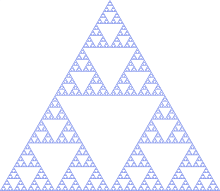
\includegraphics{SG.png}};
			\node at (0,-0.85) {The End};
		\end{tikzpicture}
	\end{center}
\end{frame}

\end{document}